\section{Methodology}
\label{sec:method}

%%----------------------------------------------------------------
%% Overview Figure
%%----------------------------------------------------------------
\begin{figure*}[t]
	\begin{center}
	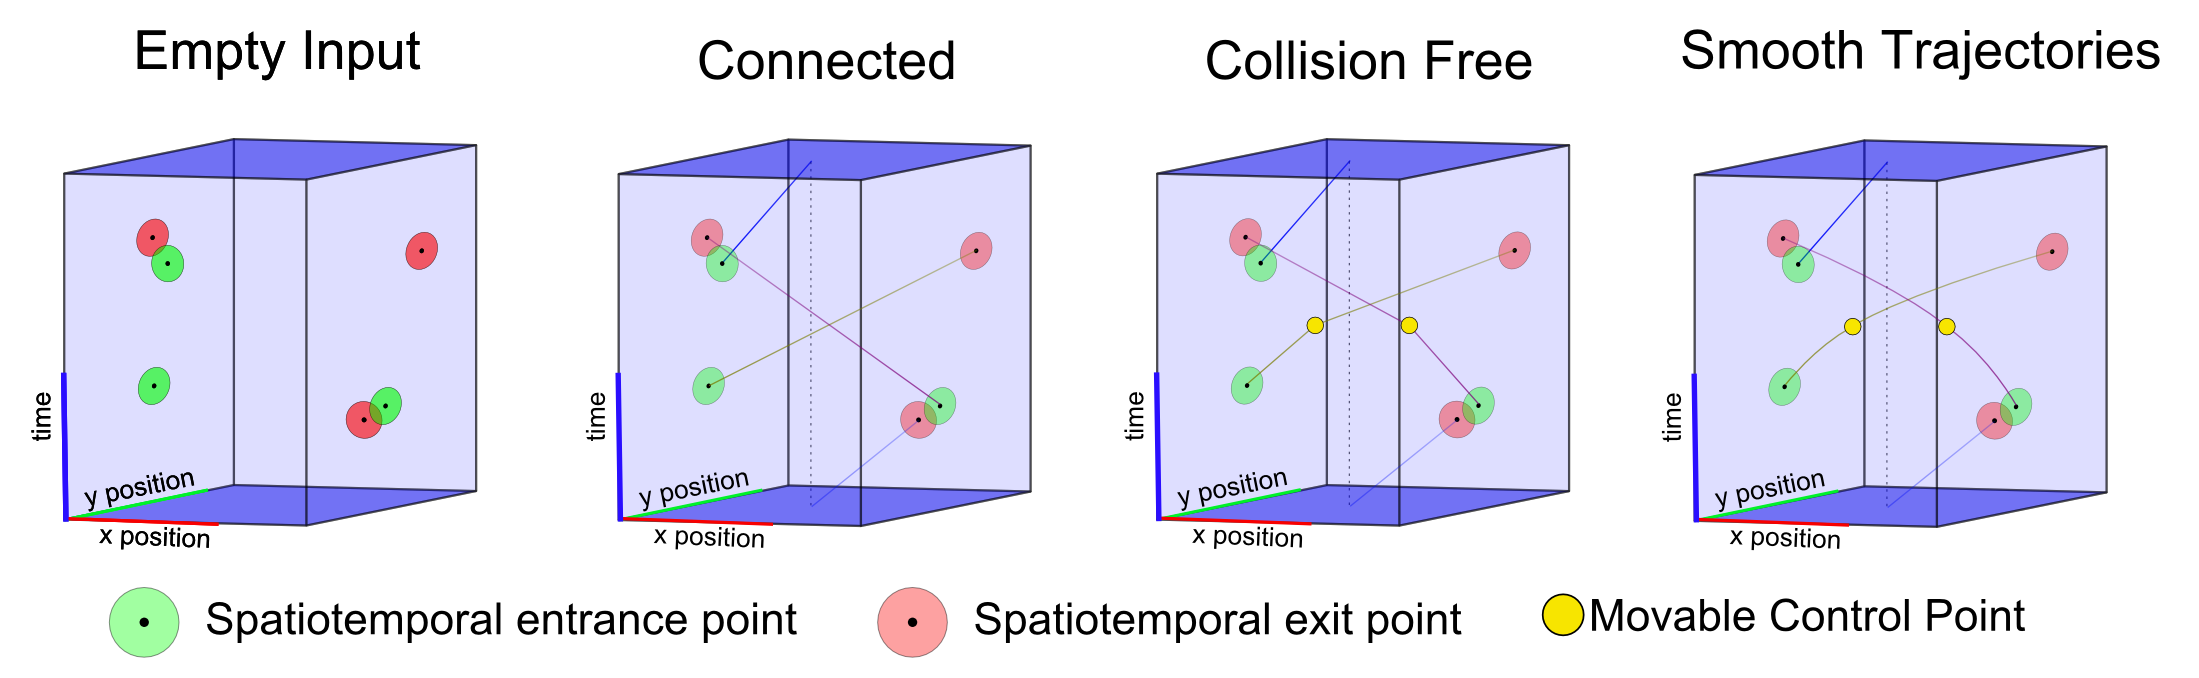
\includegraphics[width=0.9\linewidth]{./images/overview-hd.png}
% 	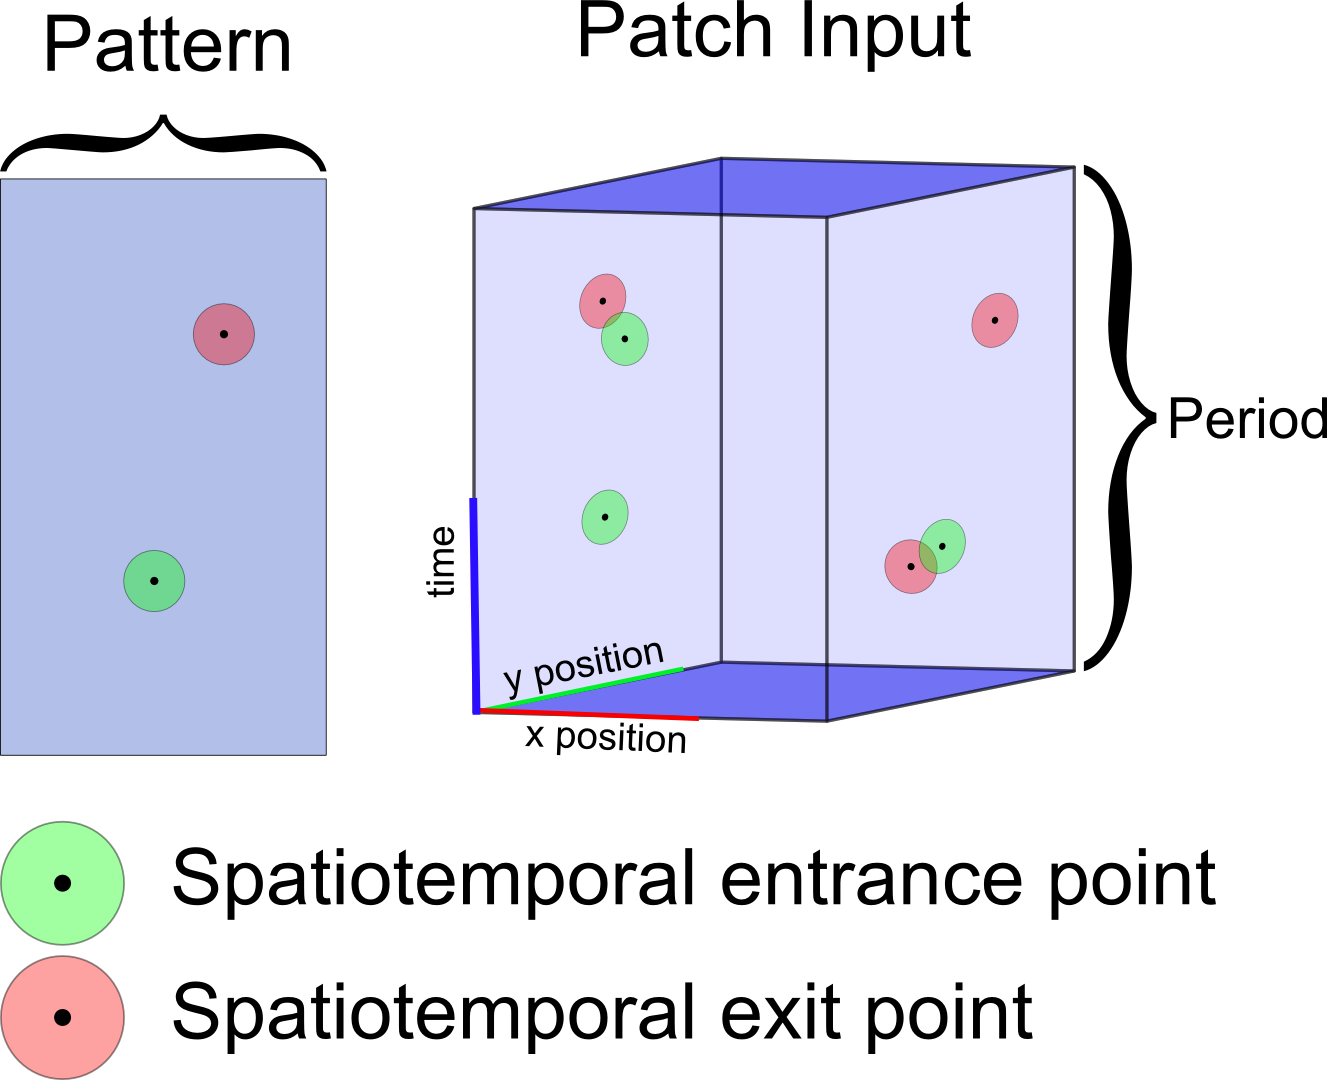
\includegraphics[height=4cm]{./images/patches-empty-patch-with-pattern.png}
% 	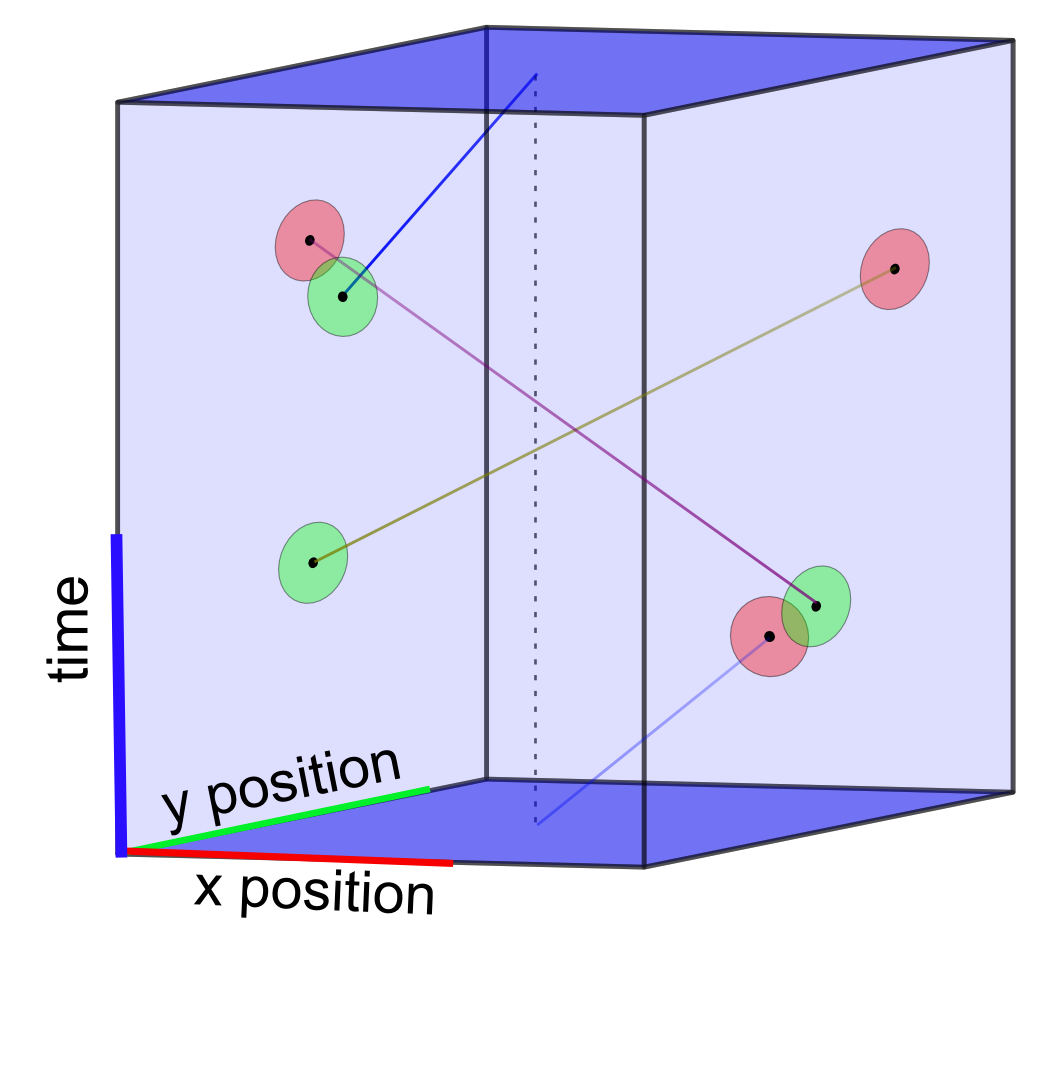
\includegraphics[height=4cm]{./images/patches-connected-patch.png}
% 	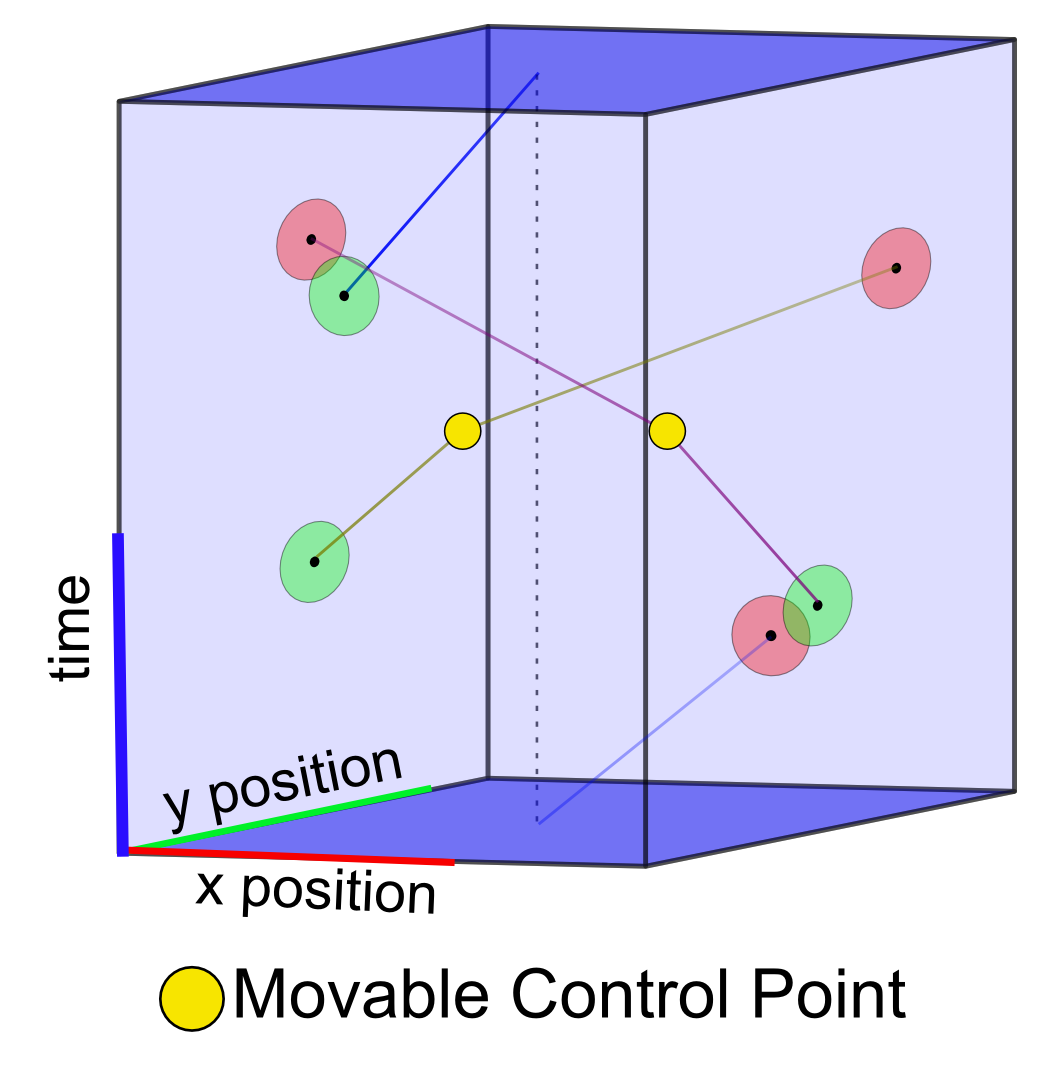
\includegraphics[height=4cm]{./images/patches-collision-free-patch.png}
% 	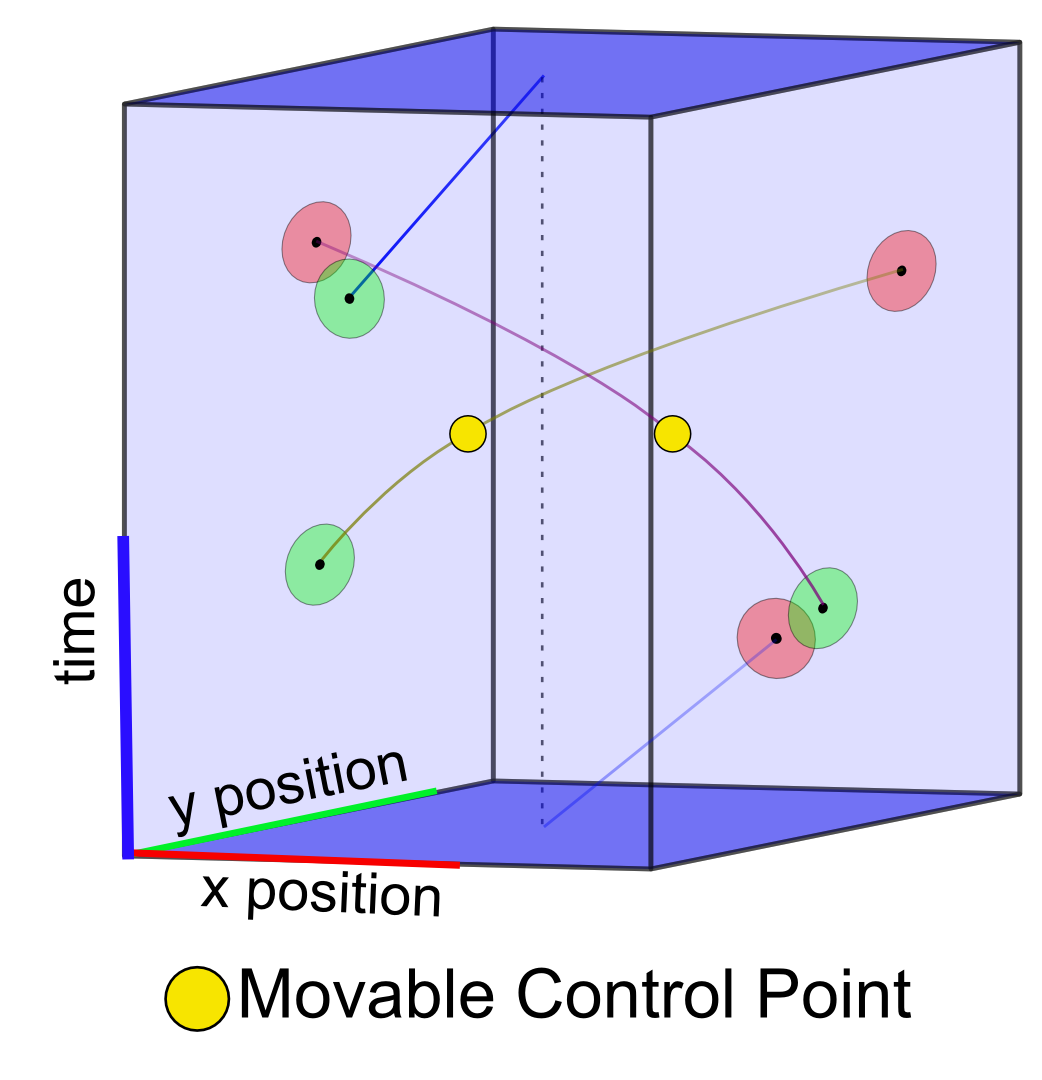
\includegraphics[height=4cm]{./images/patches-smoothed-patch.png}
	\caption{
		\textbf{Overview} Input and output points in a patch's patterns are initially connected and subsequently modified using the proposed optimization approach and smoothed out to be collision free.
	}
	\label{fig:overview}
	\end{center}
\end{figure*}
%%----------------------------------------------------------------
%% Overview Figure
%%----------------------------------------------------------------

%\note{Overview: remind definitions on crowd patches: patch, pattern, spatiotemporal waypoints (boundary conditions: input, output, initial states // boundary conditions should be strictly enforced. Movable control points), period of time \dots}

In this section we present the proposed methodology for generating trajectories for patches.
We first give some definitions and notations (Section~\ref{sec:method:definitions}), followed by an overview of the method (Section~\ref{sec:method:overview}), and trajectories initial generation, collision handling and smoothing out (Sections~\ref{sec:method:init}--\ref{sec:method:smoothing}).

%%===============================================================
%% Subsection: Patch Definitions
%%===============================================================
\subsection{Definitions}
\label{sec:method:definitions}

Before presenting our approach on trajectory generation for Crowd Patches, we present some definitions and notations regarding Crowd Patches.
Please refer to Figure~\ref{fig:definitions} for a visual representation of the definitions and \cite{Yersin:2009} for a more detailed description.

%%----------------------------------------------------------------
%% Patch Definitions
%%----------------------------------------------------------------
\begin{figure}
\begin{center}
	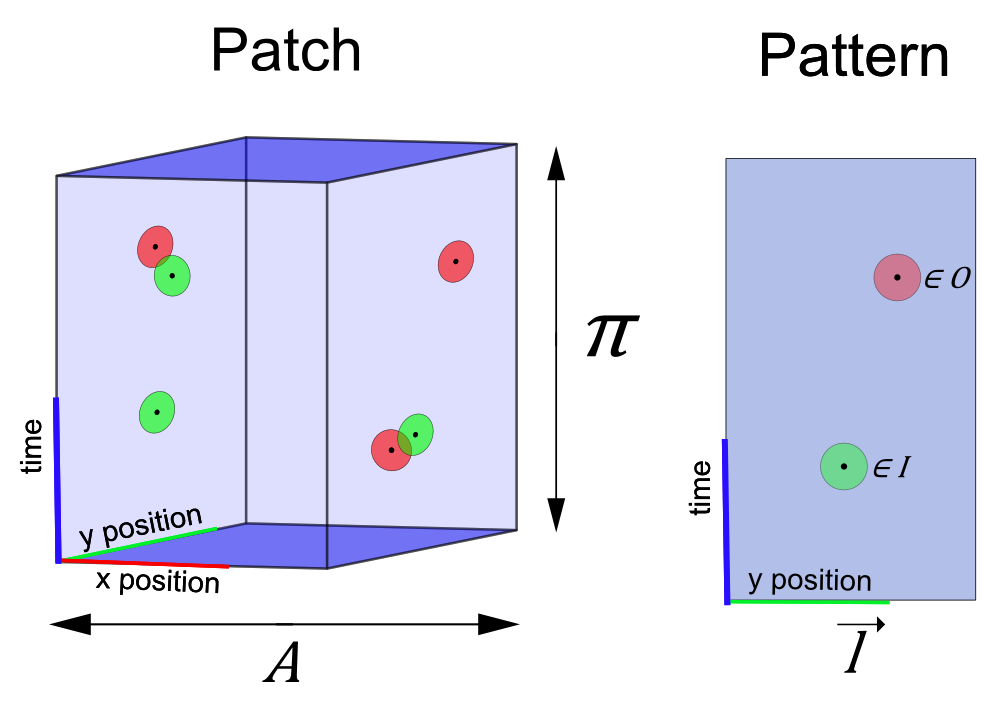
\includegraphics[width=0.9\linewidth]{./images/patch-definitions-arrows.png}
	\caption{
		\textbf{Patches and Patterns} A \emph{patch} is defined by the geometrical area $A$ where a set of dynamic and static objects ($D$ and $S$ respectively) can move over a period of time $\pi$. \emph{Patterns} define boundary conditions for the patches and act as portals connecting neighboring patches. 
	}
	\label{fig:definitions}
	\end{center}
\end{figure}
%%----------------------------------------------------------------
%% Patch Definitions
%%----------------------------------------------------------------
 
%\begin{description}

%\item[Patch]{
A \textbf{patch} is a set $\{ A, \pi, D, S\}$ where $A$ is geometrical area with a convex polygonal shape, $\pi$ the period of time of the animation and $D$ and $S$ are the sets of dynamic and static objects, respectively. 
These last two sets may be empty in case of an empty patch.
%This implies that objects in sets $D$ and $S$ move in the area defined by $A$ over some period in time $[t_1, t_2]: 0\le t_1 < t_2 \le \pi$. 
%}

%\item[Static obstacles]{
\textbf{Static objects} are simple obstacles whose geometry is fully contained inside the patch.
%}

%\item[Dynamic objects]{
\textbf{Dynamic objects} are animated; i.e., they are moving in time according to a set of trajectories $T$.
%}

%\end{description}

\subsubsection{Trajectories}

We define a {\bf trajectory} inside a patch as a function $\tau(t)$ going from time to position, more specifically from a subset of $[ 0,\pi ]$ to $A$:

\begin{equation}
	\tau:[t_1,t_2]\rightarrow A, \hspace{0.3cm} 0 \leq t_1 < t_2 \leq \pi
	\label{eqn:trajectory}
\end{equation}

We represent a trajectory as a list of control points connected by segments:

\begin{itemize}
  \item A {\bf control point} is a point in space and time $\mathbf{cp} = \{\mathbf{p}_{cp}, t_{cp}\}$.
All control points in a trajectory can either be boundary or movable ones.
Boundary control points serve as entry and exit points to the patch and cannot be moved, added or deleted.
Movable control points on the other hand can be moved, added, or removed from the trajectory as long as they do not violate the constraints of the patch; i.e., their positions must lie inside area $A$~($\mathbf{p}_{cp} \in \mathbf{A}$) and their time $t_{cp}$ must be between $t_1$ and $t_2$.
 \item A {\bf segment} is a straight line connecting two control points in a specific order. Since these are unidirectional lines in space-time, it is important to remember that they are not allowed to go backwards in time.  
\end{itemize}


There are two categories of dynamic objects: endogenous and exogenous agents.
{\bf Endogenous agents} remain inside $A$ for the total period of time $\pi$.
In order to achieve periodicity for the animation, they are associated with a trajectory $\tau : [0,\pi] \rightarrow A$, such that it respects the periodicity condition: the position at the start and at the end of the animation must be the same, i.e. \mbox{$\tau (0) = \tau (\pi)$}.

{\bf Exogenous agents} on the other hand go outside $A$.
They enter the patch at time $t_{initial}$ and position $\mathbf{p}_{initial}$, and they exit at time $t_{final}$ and position $\mathbf{p}_{final}$.
For each agent we associate a sequence of $n \ge 1$ trajectories $\{ \tau_1, \tau_2, \dots, \tau_n\}$.
Sequences may have only one trajectory, but some agents require additional trajectories in order to satisfy speed and time constraints.
The following conditions must be respected in each sequence of trajectories associated with an exogenous agent:

\begin{enumerate}
	\item $\mathbf{p}_{initial}$ and $\mathbf{p}_{final}$ must be points on the borders of $A$ otherwise they cannot be exogenous agents.
	\item If the sequence is composed by more than one trajectory, for each two contiguous trajectories, the following must be true to ensure continuity: $\tau_i(\pi) = \tau_{i+1}(0)$.

\end{enumerate}

Note that the second condition implicitly implies that in sequences with multiple trajectories, each middle trajectory must be fully defined in the period of time $[0,\pi]$, while $\tau_1$ must be defined in $[t_{initial},\pi]$ and $\tau_n$ must be defined in $[0, t_{final}]$.


\subsubsection{Patterns}

% \begin{description}
% 
% \item[Pattern -]{
A patch can be considered as a spatio-temporal right prism depending on the type of polygon used as its area (cube in the case of a squared area patch).
A \textbf{pattern} can be defined as one lateral side of the prism (Figure~\ref{fig:definitions}).
Specifically, it is a rectangle whose base is one of the edges of the polygonal area (we define $\mathbf{l} \in \mathbb{R}^2$ as this two dimensional vector), and its height is equal to the period $\pi$.
In addition to these, patterns also include the sets $\mathbf{I}$ and $\mathbf{O}$ of Input and Output boundary control points respectively.
The input set contains the boundary control points where exogenous agents begin their trajectories; we call these \emph{Entry Points}.
Conversely the elements of output are called \emph{Exit Points}; they establish the position in time and space that the exogenous agents finish their paths.
Formally defined, a pattern $\mathbf{P}^{(i)}$ is:

\begin{equation}
% 	\mathbf{P}_i = \{\mathbf{l}_i, \pi, I_i [p_i, t_i], O_j[p_j, t_j]\}
	\mathbf{P}^{(i)} = \{\mathbf{l}^{(i)}, \pi^{(i)}, \mathbf{I}^{(i)}, \mathbf{O}^{(i)}\}
\end{equation}

To populate virtual environments, patches are concatenated together.
Thus, continuity between trajectories should be enforced for exogenous agents passing through two contiguous patches.
This means that two adjacent patches must have a similar pattern on the side they share; i.e., the vector $l$ and period $\pi$ must be the same and the input and output sets must be exchanged.
More formally, having two patterns $\mathbf{P}_1$ and $\mathbf{P}_2$ where
$P^{(1)}=\{\mathbf{l}^{(1)}, \pi^{(1)}, \mathbf{I}^{(1)}, \mathbf{O}^{(1)}\}$ and~
$P^{(2)}=\{\mathbf{l}^{(2)}, \pi^{(2)}, \mathbf{I}^{(2)}, \mathbf{O}^{(2)}\}$, then, in order to satisfy $C^0$ continuity the following must apply:

\begin{equation}
	l^{(1)}=l^{(2)}, \pi^{(1)}=\pi^{(2)}, \mathbf{I}^{(1)} = \mathbf{O}^{(2)}, \mathbf{I}^{(2)} = \mathbf{O}^{(1)}
% 	\forall \mathbf{cp}_i \in \mathbf{I}^{(1)} \exists \mathbf{cp}_o \in \mathbf{O}^{(2)}
\end{equation}

Under these conditions, $P_1$ is the mirror pattern of $P_2$ and vice versa.
When these patches are animated, this will be observed as moving agents going from one patch to adjacent ones. 
If the area $\mathbf{A}$ of a patch is a square then 4 patterns are defined, one per side.
Patterns defined by a patch have the property that the sum of the cardinality of all the inputs is the same as the sum of the cardinality of all outputs; we call this the parity condition: $\sum(|inputs|)= \sum(|outputs|)$.

A patch defines a set of patterns, and conversely, a set of patterns that satisfies the parity condition;i.e. all patterns in the set have same period and whose vectors define a convex polygonal area, can be used to create a patch indirectly.

%  }
% 
% \end{description}

%%===============================================================
%% Subsection: Method Overview
%%===============================================================
\subsection{Overview}
\label{sec:method:overview}

The objective of the proposed work is to generate a patch given a set of patterns.
This implies that given a set of constraints such as input and output spatio-temporal control points, a set of believable collision-free trajectories should be generated that interconnect all of them.
This process has three main steps (Figure~\ref{fig:overview}):
\begin{enumerate}
  \item Match the elements in the Input and Output sets contained within a patch.
  In this step, Entry to Exit Points are connected based on a score function that tries to keep agents close to their preferred speed while at the same time avoiding connections to similar patterns, thus reducing unwanted u-turns.
  The input for this step is a set of patterns and the output is a set of piecewise linear trajectories connecting the entry and exit points.
  \item Create collision free trajectories for these pairings.
  Starting from simple line trajectories; these are bended iteratively until they are collision free.
  %W0e0 start with simple line trajectories and start bending them until they are collision free.
  Points lying at the borders, i.e. Entry and Exit points, are hard restraints and can never be moved.
  \item Smooth out trajectories (if needed).
   Lastly splines are used to minimize the hard turns making sure that the smoothed out trajectories stay as close as possible to the original ones from step $2$ so that no new collisions are introduced.
%    We make sure the new trajectories stay close to the original ones, lest we create new collisions.
\end{enumerate}

% \note{Problem : is to compute internal trajectories that join all boundary conditions with conitnuous and believable motion trajectories. 
% 
% 2 steps: 
%  - step 1: connect waypoints
% INPUT first boudnary conditions are ``alone'' in patches $\rightarrow$ associate/connect waypoints
%  them 
% OUTPUT : initial trajectories (piecewise linear trajs, possibly colliding, with ``good'' properties that we will define later on)
% 
%  - step 2: optimize intial trajectories by moving control points to remove collisions
%     INPUIT : initial trazjectories
%       OUTPUT : colliision trajectories, still enforcing boundary conditions
%       
% - step 3 is smoothing
% }       

A more detailed look on all three steps is given over the remainder of this section.

\subsection{Connecting Boundary Control Points}
\label{sec:method:init}

The first step to the proposed algorithm is to match all the entry and exit points in an optimal way.
To do this, a measure of the match's quality has to be defined.
%we have to measure how good or bad a match is.
Intuitively, there are some matches that are better than others; e.g., judging by observation, trajectories passing near the center of the patch look better that the ones staying close to the borders forcing in essence the characters to cover more space.
Some other aspects can also be considered, such as how close the speed needed by an agent to travel from an Entry to an Exit Point is compared to typical walking comfort speeds of humans.
A comfort speed of $u_{cft} = 1.33~m/s$, which is the normal walking speed of humans in an unconstrained environment is used in this work \cite{Whittle2003Gait}.

For a square patch, we define an order of preference between matching; first we prefer to match points between opposing patterns, followed by neighboring ones and finally with points on the pattern itself.
%Then the points on the contiguous pattern and finally, the points that are in the same pattern.
For any of these cases, if there exist multiple possible matching options on the same pattern, the point whose associated trajectory is closest to the defined comfort speed is selected.

To solve this matching problem, we employ the \emph{Gale-Shapley algorithm}~\cite{gale1962college} (see Algorithm~\ref{alg:stable-matching}), commonly referred to as the algorithm to solve the \emph{stable marriage problem}. 
This algorithm assures that at the end, if we have Alice engaged to Bob and Carol engaged to Dave, it is not possible for Alice to prefer Dave and Dave to prefer Alice -- this is called a \emph{stable match}.  

Algorithm~\ref{alg:stable-matching} demonstrates the Gale-Shapley algorithm in relation to two equal lists of men and women who are being matched for marriage.
However the algorithm generalizes to any matchable objects, which in our case are entry and exit points.

%%-------------------------------------------------------------------
%% The Stable Marriage Algorithm by Gale-Shapley
%%-------------------------------------------------------------------
\begin{algorithm}[t]

Initialize all $m \in M$ and $w \in W$ to \textit{free} \;
\While {$ \mathbf{\exists}$ \textit{free} man $m$ who still has a woman $w$ to propose to} {
	$w \leftarrow m's$ highest ranked woman to whom he has not yet proposed \;
	\eIf {$w$ is \textit{free}}
	{ 
		$(m,w)$ become engaged \;
	}
	{
		some pair $(m',w)$ already exists \;
		\eIf {$w$ prefers $m$ to $m'$} 
		{
			$(m,w)$ become engaged \;
			$m'$ becomes \textit{free} \;
		}
		{
			 $(m',w)$ remain engaged;
		}
	}
}
\caption{Gale-Shapley Stable Marriage Algorithm from \cite{Gusfield1989SMP}.}
\label{alg:stable-matching}
\end{algorithm}
%%-------------------------------------------------------------------
%% The Stable Marriage Algorithm by Gale-Shapley
%%-------------------------------------------------------------------


% All that is needed to use this algorithm is to generate preference values for entry and exit points.
% For each of the entry Entry points, the following steps are appliedThis is done using the following steps:
In order to apply Algorithm~\ref{alg:stable-matching}, preference values for all combinations of entry and exit points should be defined.
To do so, each entry point keeps a \emph{proposal list} $\mathbf{L}_s$ indicating order of preference for matching (Figure~\ref{tab:proposal-list}).
The following approach is employed to rank each possible matching:
\begin{enumerate}
  \item Find the speed it would take to travel from an entry point to all exit points.
  Assuming that $(\mathbf{p}_1, t_1)$ and $(\mathbf{p}_2,t_2)$ are position and time of the entry and exit points respectively
  speed is defined as $u = s / {\Delta}t$ where $s=|\mathbf{p}_2-\mathbf{p}_1|$ and ${\Delta}t = t_2 - t_1$ when $t_2 > t_1$, otherwise ${\Delta}t=\pi + t_2 - t_1$.
  \footnote{More details on why this this last assumption is made will be presented later during the creation of the initial set of trajectories.}
  \item %Next, each pair of points is assigned a number between $0$ and $\pi/2$, with $0$ indicating maximum closeness to comfort speed with $arctan(|u_{cft} -u|)$.
  Next, each pair of points is assigned a preference value:
  \begin{equation}
  	pr_{score} = u_{match} + p
  	\label{eqn:objective_function}
  \end{equation}
  where
  		$u_{match} = arctan(|u_{cft} - u|) \in [0, \pi / 2)$ indicates closeness to desired speed with $0$ indicating maximum closeness. 
    	$p = \{0, 2, 4\}$ defines a \emph{penalty} value that depends on where the two points lie relative to each other; for points on opposing patterns there is no penalty, for neighboring patches it is $2$ and for points on the same pattern it is $4$ (this can be generalized to any prism like patch). 

  % and We add penalties for points being in the same patch, for those points, we add $4$. For points lying in the contiguous pattern we also add a smaller penalty, $2$.
  \item Sort $\mathbf{L}_s$ in ascending order; the first entry indicates the most desired exit point.
\end{enumerate}
 

%%-------------------------------------------------------------------
%% The Proposal List table
%%-------------------------------------------------------------------
\begin{table}[b]
	\centering
	\caption{
	\textbf{Proposal List} Each entry point keeps a list of preference scores for all possible Exit points.
	Lower values indicate bigger preference, with exit point B in this case being the most preferred one.
	Exit Points F and D lie in the same pattern as Entry Point $1$, so they receive a higher number.
	}
	\begin{tabular}{c|c}
% 		\multicolumn{2}{c}{Rankings of preferred}\\
% 		\multicolumn{2}{c}{partners for Entry Point A}\\
		\hline
		\multicolumn{2}{c}{Entry Point: $1$}	\\
 		\hline
 		\hline
		Exit Point	&	Preference\\
		\hline
% 		\hline
		B	&	$\mathbf{0.34}$	\\
		C	&	$1.3$			\\
		A	&	$2.3$			\\
		E	&	$2.4$			\\
		D	&	$4.5$			\\
		F	&	$4.6$			\\
		\hline
		\end{tabular}
	\label{tab:proposal-list}
\end{table}
%%-------------------------------------------------------------------
%% The Proposal List table
%%-------------------------------------------------------------------

It is emphasized here, that each entry point keeps its own proposal list.
After each entry point has been assigned a proposal list, Algorithm~\ref{alg:stable-matching} is used to define matches between the entry and exit points;
every two points that remained engaged at the end of the algorithm become a pair.

The final step is creating the initial batch of trajectories.
Firstly, the paired points are connect with straight lines;
% We start by trying to connect the points with a straight line.
if a line tries to connect two points backwards in time (that is if $t_2 < t_1$), the initial trajectory is split into two parts -- from $t_1$ to $\pi$ and from $0$ to $t_2$; similarly to approach followed by \cite{Yersin:2009}.
% We do something special when a line tries to travel backwards in time, i.e. $t_2<t_1$.
% For these cases we split the initial trajectory in two.
% One going from $t_1$ to period $\pi$, another one going from $0$ to $t_2$.
The positions of these new control points are in the same straight line, taken in such a way that the speed is the same in both segments.
The same approach is used if the trajectory enforces unrealistically high speed values ($u \gg u_{cft}$).

Further adjustments to the initial trajectories are done for some special cases.
For agents traveling only over an edge, a control point is added near the center of the patch.
For agents moving slowly a control point with the same position but on a different time is added, resulting in agents that stop suddenly (as if pausing to look around) but later on continuing their journey at a better speed.

% \devin{The output of this function is a set of trajectories. Collisions are probably still present in the trajectories at this point.}
 
 To conclude, this step results in linear trajectories that are optimized for speed and coverage of space using an objective function (Equation~\ref{eqn:objective_function}).
 These trajectories though can result in collisions, since no special care was taken to handle that.
 To do so, an iterative approach has been proposed.

% \note{
% - INPUT OUTPUT objective
% 
% - when you connect two boundary conditions, you connect two spation temporal waypoints. This means that you determine this way where characters enter, where they exit patches and the speed between waypoints. 
% 
% - we can define what is a ԧoodԠconnection: avoid half turn, avoid extreme speeds. 
% 
% - we define an objective function, we solve this using the stable marriage problem. 
% 
% - reminder of 2009 paper - you explain the specific case of splitting trajectories. 
% 
% -  you provide pseudo algo for this,  
% 
%  - you define all the variables/parameters you use. 
%  
% summarize what you get as an aoutput, and what is the next step.
% }
% 

%%===============================================================
%% Subsection: Removing Collisions
%%===============================================================
\subsection{Removing Collisions}
\label{sec:method:remove-collisions}

%\panayiotis{Make sure for all the equation that the correct symbols are inserted: bold for vectors, normal fonts for scalars, etc.}
Most of the times, the set of linear trajectories generated by Algorithm~\ref{alg:stable-matching} have collisions and therefore care should be taken to remove them since collisions rarely occur in real life human crowds.
An algorithm that manipulates the linear trajectories by moving control points is proposed.
Since patches are concatenated together to create larger crowds care should be taken during trajectory modification so that the spatio-temporal boundary control points (i.e., entry and exit ones) are not modified; other control points can be added and manipulated.
% The removal procedure must handle collisions by manipulation of the trajectories aiming to keep the spatio-temporal entrance and exit points (boundary control points).

% These trajectories contain both movable and boundary control points; 
% We are given a set of trajectories within a patch consisting of both movable and boundary control points.
% What we expect in return is modified trajectories that have maintained their spatio-temporal entrance and exit points while removing all collisions throughout the entire period of the patch.
%Our objective is to use these patches in larger crowd simulations of people.
%We would like to create trajectories that could represent human motion.
%We focus on creating collision free motion since obvious collisions in simulations greatly reduces the realism of the animation.

\textbf{Algorithm for collision handling} An iterative algorithm for handling the collisions is proposed (Algorithm~\ref{algo:control-points}).
The main idea is simple; given a matrix $M$ that stores the current minimum distances in-between all trajectories iterate modifying trajectories (and therefore $M$) until $min(M) > \theta$, where $\theta$ represents a minimum allowed distance value.
Given typical circular agents of radius $r$, $\theta = 2r$ (therefore iff $min(M) > \theta \Leftrightarrow \text{patch is collision free}$).
To do so, new control points are added in each iteration (i.e., trajectories are split into segments) that are moved under some constraints until the trajectories are collision free.

% Our algorithm (see Algorithm~\ref{algo:control-points}) creates collision free trajectories by adding and modifying control points. We can guarantee this by looking at the minimum distance matrix. If every value in the matrix is above some threshold then we know that for the entire period of the patch no two agents come closer than that threshold. So if we make that threshold equal to the sum of the radii being compared, those agents will never touch.


%%-------------------------------------------------------------------
%% Removing collisions figure
%%-------------------------------------------------------------------
\begin{figure*}[t]
	\begin{center}
	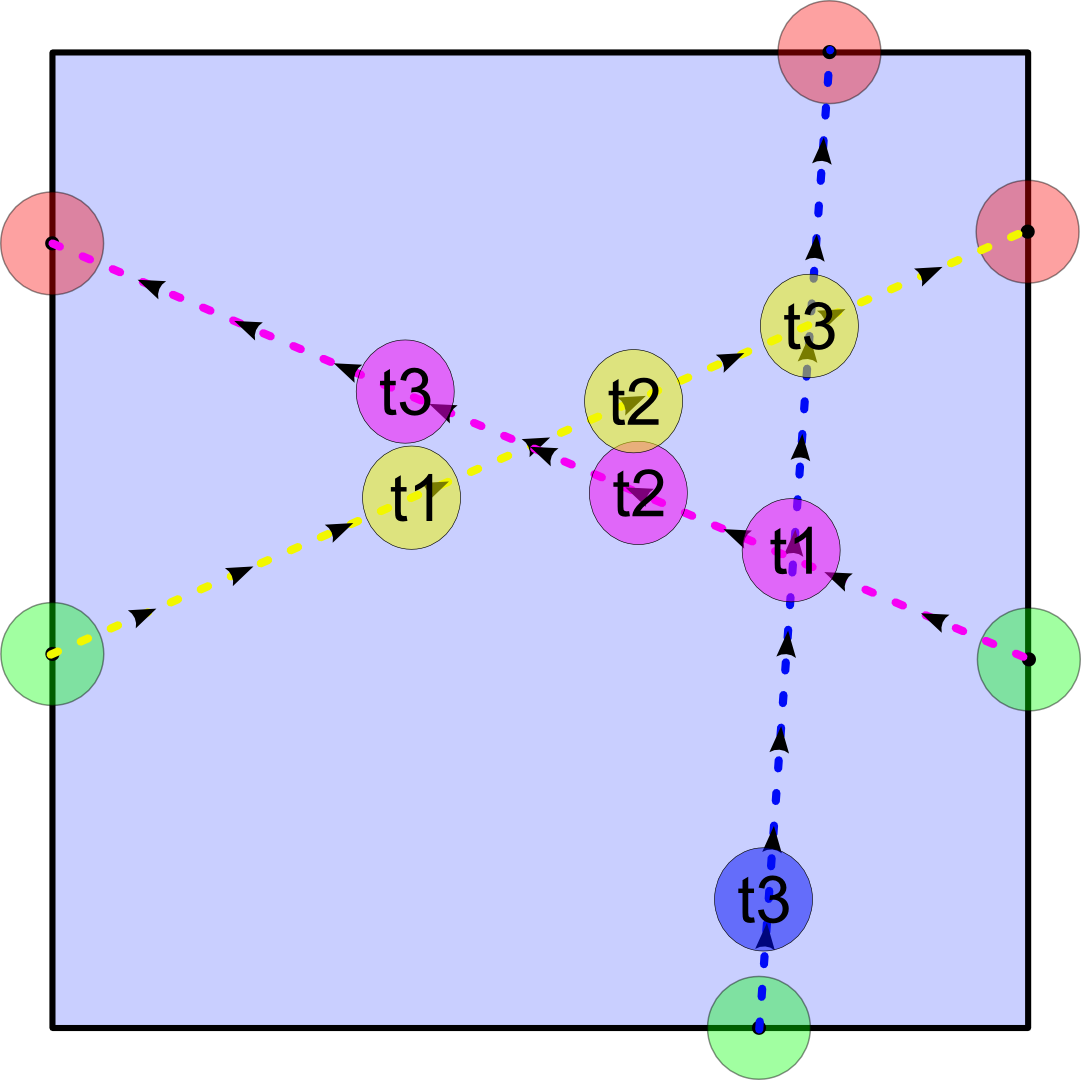
\includegraphics[width=0.3\linewidth]{./images/collision-2D-example-with-collision.png}
	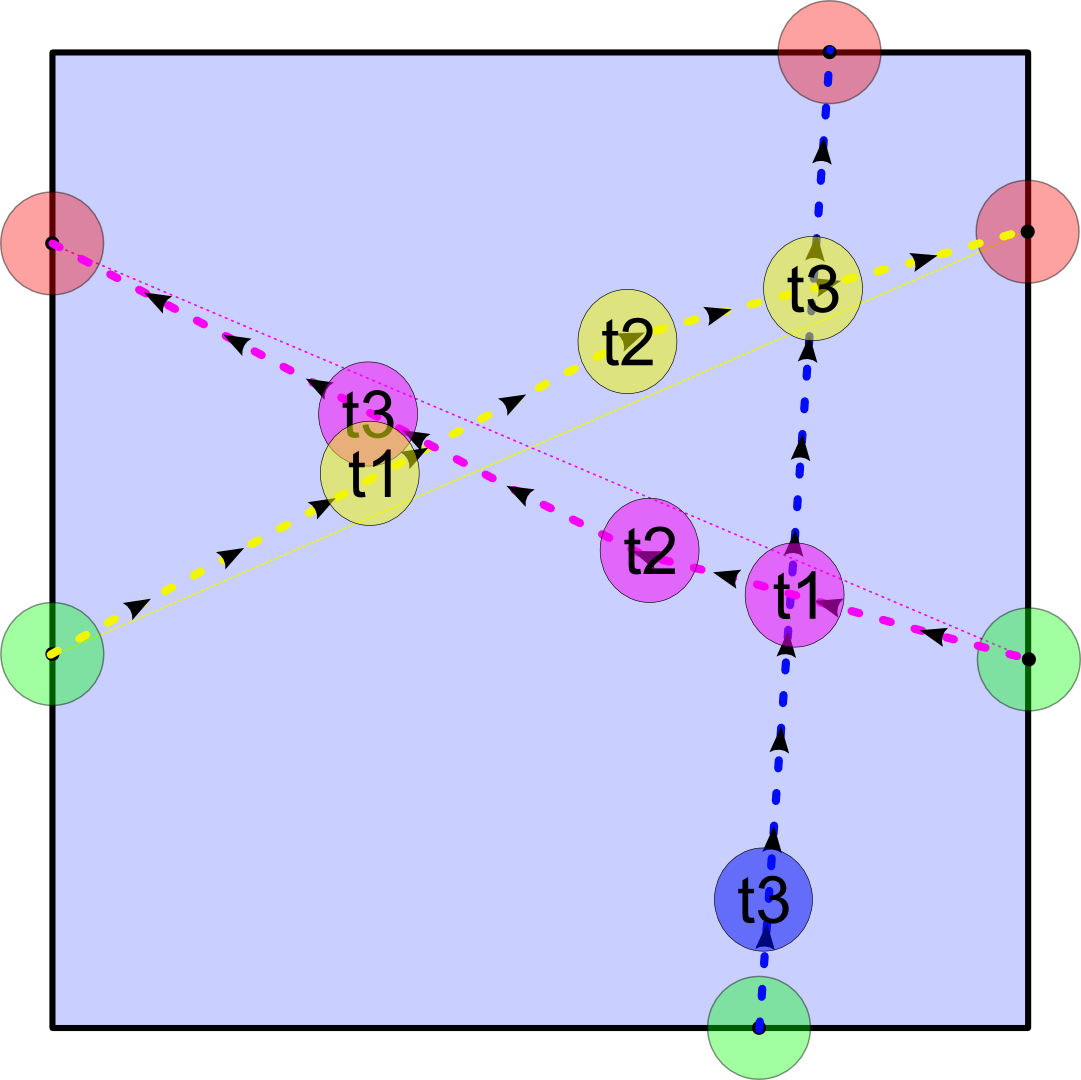
\includegraphics[width=0.3\linewidth]{./images/collision-2D-example-without-collision.png}
	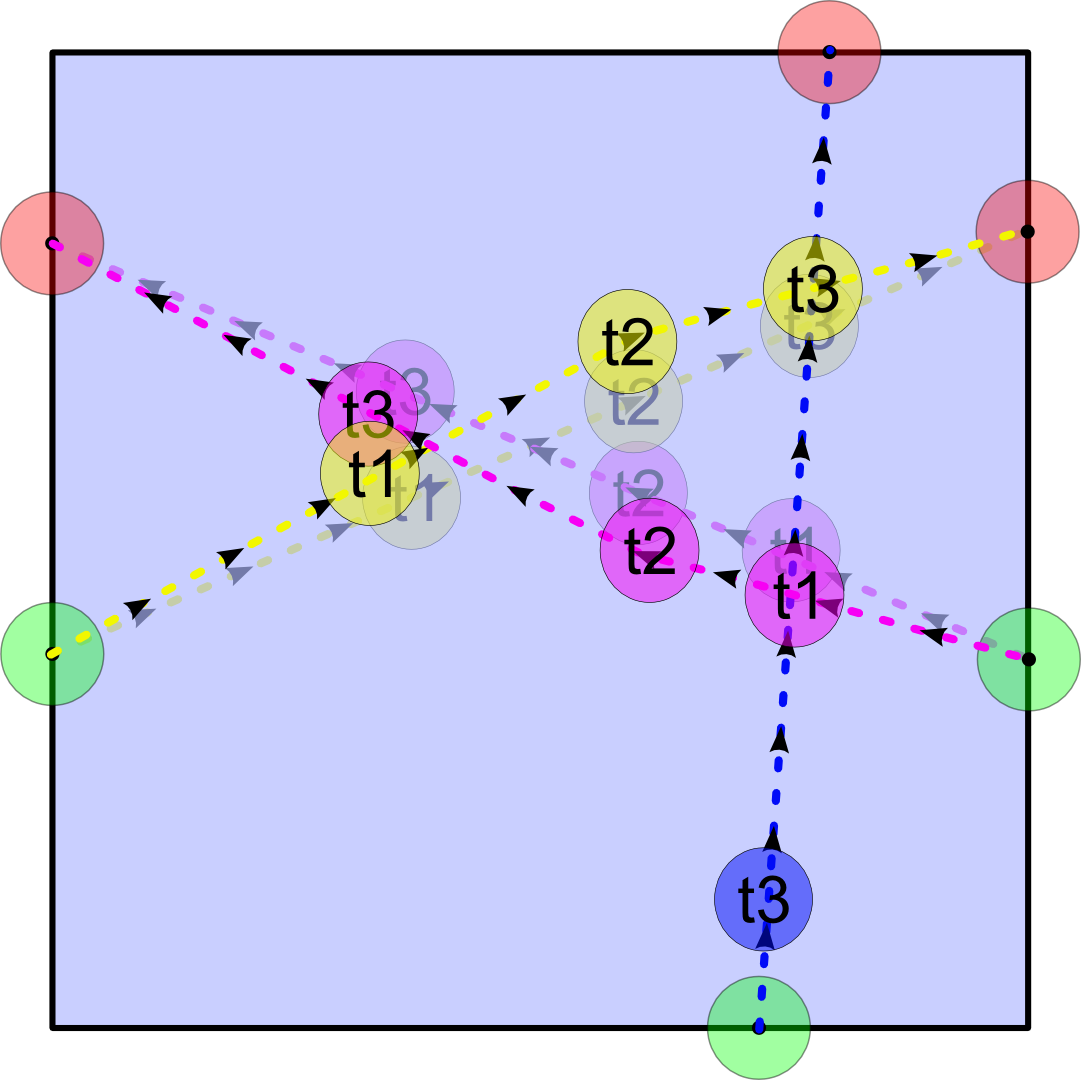
\includegraphics[width=0.3\linewidth]{./images/collision-2D-example-overlay.png}
	\\
	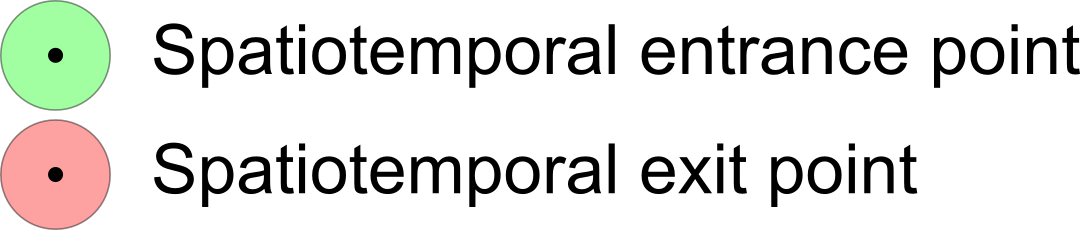
\includegraphics[width=0.3\linewidth]{./images/key-entry-exit-point.png}
	\caption{
		\textbf{\textbf{Collision removal}}
	}
	\label{fig:collision-removal}
	\end{center}
\end{figure*}
%%-------------------------------------------------------------------
%% Removing collisions figure
%%-------------------------------------------------------------------



%%-------------------------------------------------------------------
%% Control Points algorithm
%%-------------------------------------------------------------------
\begin{algorithm}[t]
% \hline
% \vspace{0.1cm}
Compute minimum distance matrix $M$\;
\While{there exists at least one entry in $M$ below the threshold}{
	Find indices $i$  and $j$ for which $M(i,j)$ has the smallest value $d$\;
	Create temporary control points $\mathbf{cp}_i$ and $\mathbf{cp}_j$ in $\tau_i$ and $\tau_j$ that are at distance $d$ \;
	Apply repulsion forces to $\mathbf{cp}_i$ and $\mathbf{cp}_j$\;
	Update  $\tau_i$ and $\tau_j$\;
	Update $M$ \;
	}
\caption{The control points generation algorithm}
\label{algo:control-points}
\end{algorithm}
%%-------------------------------------------------------------------
%% Control Points algorithm
%%-------------------------------------------------------------------





First, the minimum distance matrix is calculated (Section~\ref{sec:method:remove-collisions:distance-matrix}).
As long as collisions exist, trajectories $\tau_i$ and $\tau_j$ having the minimum value are found -- that minimum value corresponds two a moment in time and two points: $\mathbf{p}_i$ and $\mathbf{p}_j$.
These two points are moved to handle the collision using correction forces $\mathbf{F}_i$ an $\mathbf{F}_j$:

\begin{equation}
	 \mathbf{F}_{i}= R(\phi) * \hat{\Delta{\mathbf{p}_{i, j}}}* \theta * w_i
\end{equation}

$\hat{\Delta{\mathbf{p}_{i, j}}}$ is the normalized distance vector between the two points ($\Delta{\mathbf{p}_{i, j}} = \mathbf{p}_i - \mathbf{p}_j)$),
$\theta = r_j + r_j$ is the sum of the two agents' radii and defines a threshold value for minimum distance\footnote{In our implementation $r_1 = r_2 = r$, making the threshold constant.},
$R(\phi)$ is a small random noise rotation matrix to help prevent infinite loops ($\phi: -0.5 \le \phi \le 0.5 \hspace{0.1cm} rad$),
an finally $w_i$ and $w_j$ are weights to reduce speed artifacts and prevent agents from leaving the bounds of the patch:

\begin{equation}
w_i = \left\{
	\begin{array}{l l}
		u_j / (u_i + u_j)	&	\quad \text{if point stays in patch}\\
		0					&	\quad \text{otherwise}
	\end{array}
	\right.
\end{equation}

$u_i$ and $u_j$ are the speeds of trajectories $\tau_i$ and $\tau_j$.

Having the correction force, point $\mathbf{p}_i$ is moved according to the following equation:

\begin{equation}
	\mathbf{p}_i^{new} = \mathbf{p}_i + \mathbf{F}_i
\end{equation}


Once $\mathbf{p}_i^{new}$ is found, a check to find if there is an existing control point withing a small time interval is performed; if successful, then the existing control point is moved to $\mathbf{p}_i^{new}$ otherwise a new control point is added at the same position.
Finally, column $i$ and row $j$ of the distance matrix $M$ are updated with new distances.
Calculations for force $\mathbf{F}_j$ and point $\mathbf{p}_j$ are symmetric.

We find that in many situations this algorithm converges quickly and produces collision free trajectories (Section~\ref{sec:results}).
However there are still situations where it converges slowly or even gets stuck in an infinite loop; for these a maximum number of iterations is set.


\subsubsection{Distance Matrix Calculation}
\label{sec:method:remove-collisions:distance-matrix}
\textbf{Distance Matrix} The first step of the collision handling algorithm is generating a distance matrix $M \in \mathbb{R}^{nxn}$ between all the $n$ trajectories; i.e., the value at $M(i, j)$ represents the minimum distance between trajectories $\tau_i$ and $\tau_j$ (Table~{\ref{tab:minimum-distances}}).

The following properties apply for all $i, j \in [1, n]$ and can be employed to reduce computation time:
\begin{itemize}
  \item $M(i, i) = 0$
  \item $M(i, j) = M(j, i)$, i.e., the matrix is symmetric
  \item $M(i, j) = \infty$, \hspace{0.1cm}$\forall (\tau_i, \tau_j$) that are never present at the same time
\end{itemize}

\textbf{Minimum Distance} The minimum distance between two trajectories is defined as their minimum spatio-temporal distance; i.e. the point in time where they are closer to each other.
Recall that a trajectory can consist of one or more segments separated by control points (Section~\ref{sec:method:definitions}) and therefore the minimum has to be found in-between all the trajectory's segments.

Given any two linear trajectory segments $\mathbf{s}^{(1)}$ and $\mathbf{s}^{(2)}$, their minimum distance can be found with an analytic approach.
First, their common time interval is found; i.e., the period of time that the trajectories coexist in the patch.
If the two segments did not have any common time interval, then their distance is set to infinity (practically a large value).
If there exists a common interval $[t_{s}, t_{e}]$ then we set $\mathbf{p}_s^{(1)}$ and $\mathbf{p}_s^{(2)}$
% , $\mathbf{p}_e^{(1)}$ and $\mathbf{p}_e^{(2)}$
as the two segments position at time $t_s$.
Additionally, agents moving on these two segments have a velocity of $\mathbf{v}^{(1)}$ and $\mathbf{v}^{(2)}$ respectively.
So, for any point in time $t: 0 \le t \le t_e - t_s$, their distance is:

\begin{equation}
	d(t) = || (\mathbf{p}_s^{(1)}+\mathbf{v}^{(1)} * t) -
				(\mathbf{p}_s^{(2)}+\mathbf{v}^{(2)} * t) ||
	\label{eqn:distance}
\end{equation}

Setting $ \mathbf{w} = \mathbf{p}_s^{(1)} - \mathbf{p}_s^{(2)}$ and $\mathbf{\Delta{v}} = \mathbf{v}^{(1)} - \mathbf{v}^{(2)}$ Equation~\ref{eqn:distance} becomes:

\begin{equation}
	d(t) = || \mathbf{w} + \mathbf{\Delta{v}}*t ||
	\label{eqn:distance_simple}
\end{equation}

Solving for $t$ after setting the derivative $d'(t) = 0$ we get the time of minimum distance $t_c$:

\begin{equation}
	t_c = (-\mathbf{w} \cdot \mathbf{dv}) / || \mathbf{dv} || ^ 2
	\label{eqn:distance_time}
\end{equation}

If $0 \le t_c \le t_e - t_s$, then setting $t = t_c$ in Equation~\ref{eqn:distance} the minimum distance between segments $\mathbf{s}^{(1)}$ and $\mathbf{s}^{(2)}$ is found.
If $t_c$ is outside the bounds of the segment we check the endpoints of the line segment for collision.
Having all the minimum distances between all the segments of two trajectories, finding the minimum distance is trivial (consult Table~\ref{tab:minimum-distances} for an example.

%%-------------------------------------------------------------------
%% The Minimum Distances Table
%%-------------------------------------------------------------------
\begin{table}[t]
	\centering
	\caption{\textbf{Distance Matrix} Minimum distances between 4 trajectories ($\tau_0 - \tau_3$) are updated whilst modifying the trajectories.
	At this iteration of the algorithm, the minimum distance was between trajectories $\tau_1$ and $\tau_2$ and therefore they will be modified for the next step.}
	\begin{tabular}{|c||cccc|}
		\hline
		 			& $\tau_0$		& $\tau_1$ 		& $\tau_2$	& $\tau_3$	\\
		 \hline \hline
		$\tau_0$	& $0$			&	$\infty$ 	& $8.31$	& $2.10$	\\
% 		\hline
		$\tau_1$	& $\infty$		&	$0$			& $\mathbf{0.14}$	& $7.60$	\\
% 		\hline
		$\tau_2$	& $8.31$		&	$\mathbf{0.14}$ 		& $0$		& $\infty$	\\
% 		\hline
		$\tau_3$	& $2.10$		&	$7.60$ 		& $\infty$	& $0$		\\
		\hline
		\end{tabular}
\label{tab:minimum-distances}
\end{table}
%%-------------------------------------------------------------------
%% The Minimum Distances Table
%%-------------------------------------------------------------------





% Given two trajectories you can find the distance between them at any moment in time.
% The shortest distance between trajectories is the minimum of all these distances computed over the period of the patch.
% To compute the minimum distance between two trajectories we find the minimum distance between all the segments of the trajectories and take the minimum of the minimums as our final answer.
% When looking at two segments we find the intersection of the time intervals. If the intersection is not empty, we find the minimum distance. We call the start and end time of this intersection $t_0$ and $t_1$ respectively.

% Each one of those segments represent a moving agent with an initial position $\mathbf{p}_0$ and $\mathbf{p}_1$ with velocities $\mathbf{v}_0$ and $\mathbf{v}_1$ moving in the time interval $[t_0,t_1]$. 
% 
% We can then define the distance at a certain time between the two segments with the following equation.
% 
% \begin{equation}
% 	d(t) = || (\mathbf{p}_0+\mathbf{v}_0*t) - (\mathbf{p}_1+\mathbf{v}_1*t) ||
% 	\label{eqn:distance}
% \end{equation}

% For simplicity we say $ \mathbf{w} = \mathbf{p}_0-\mathbf{p}_1$ and $\mathbf{dv} = \mathbf{v}_0-\mathbf{v}_1$, so then,
% 
% \begin{equation}
% 	d(t) = || \mathbf{w} + \mathbf{dv}*t ||
% 	\label{eqn:distance_simple}
% \end{equation}
% 
% 
% 
% We are looking for the minimum so we solve for $t$ when when the derivative equals zero.
% \begin{equation}
% 	t_c = (-\mathbf{w} \cdot \mathbf{dv}) / || \mathbf{dv} ||^2
% \end{equation}
% 
% With $t_c$, the time at which the two line segments are closest we can easily calculate the position on each of those segments, and thus the distance between them. If the time is outside the bounds of the segment we check the endpoints of the line segment for collision.





% These three properties can be used to reduce computation time.

% We compute a minimum distance between each pair of trajectories.
% We store each value in a minimum distance matrix $M$.
% The position in the matrix corresponds to the trajectory ID.
% So the value at $M(i, j)$ would be the minimum distance from trajectory $\tau_i$ to trajectory $\tau_j$.
% It's good to note that this value will be the same as $M(j,i)$.
% Furthermore $M(i,i)$ will always be zero and distance for trajectories that don't intersect in time, we set them to a number bigger than the threshold for collisions, for example $100$ for a threshold of $1$ (see Table ~\ref{tab:minimum-distances}).
% These facts can be used to reduce computation while filling out the minimum distance matrix.









\subsection{Smoothing}
\label{sec:method:smoothing}

Smoothing:
We have obtained some collision free trajectories, but they may have a jerky trajectory, so we need a final the step to smooth them. We need to take special care of how we do this, we donӴ want the trajectories to change in such a way that they make new collisions. A simple approach is to use cubic splines. Cubic splines connects every pair of points in a trajectory with a polynomial function of degree $3$:

\begin{equation}
 S(x)=a+bx+ cx^2+ dx^3
\end{equation}

In total, we will need to find the coefficients a, b, c, and d for every segment we have in our trajectory. Those coefficients are determined by continuity $C^1$ restrictions: 

For every spline associated with a trajectory between control point $\mathbf{cp}_1=(\mathbf{p}_1,t_1)$ and $\mathbf{cp}_2=(\mathbf{p}_2,t_2)$, the spline must pass through those same points, that is, $S(t_1)=(\mathbf{p}_1)$ and $S(t_2)=(\mathbf{p}_2)$.

For every two contiguous splines $S_1$ and $S_2$, for the common point they share p, the velocity must be equivalent, that is,  $S'_1(\mathbf{p})=S'_2Ҩ\mathbf{p})$.
  
This restrictions can be accommodated in a such way that they form a system of linear equations that can be solved using Cholesky decomposition.

We can not apply directly this method using our current control points. That results in trajectories that vary too much from the original, thus they may end up creating new collisions. To make the spline more similar to the original trajectory, we add new virtual control points sampled uniformly in the linear segments of the trajectories. We call these tacks. These tacks help fix the splines, because they will now pass through the control points and the tacks. Note that the more tacks we put, the closer the spline will fit to the original path.

After that, we compute the coefficients to create the splines and resample along the spline to get new control points. The new trajectory will still be composed of line segments, but since they are smaller, and following closely the path of a cubic function, to the naked eye they will look like curves. The finer the sample, the more it will look like a smooth path.

For optimization purposes, the second sampling is not taken uniformly. The trajectories are relatively straight in the middle of the the segments and have higher curvature near control points. For that reason, we take more samples around inflexion points (old control points) than far from them. These samples become the new control points that define the trajectory.

%%-------------------------------------------------------------------
%% Removing collisions figure
%%-------------------------------------------------------------------
\begin{figure}[t]
	\begin{center}
	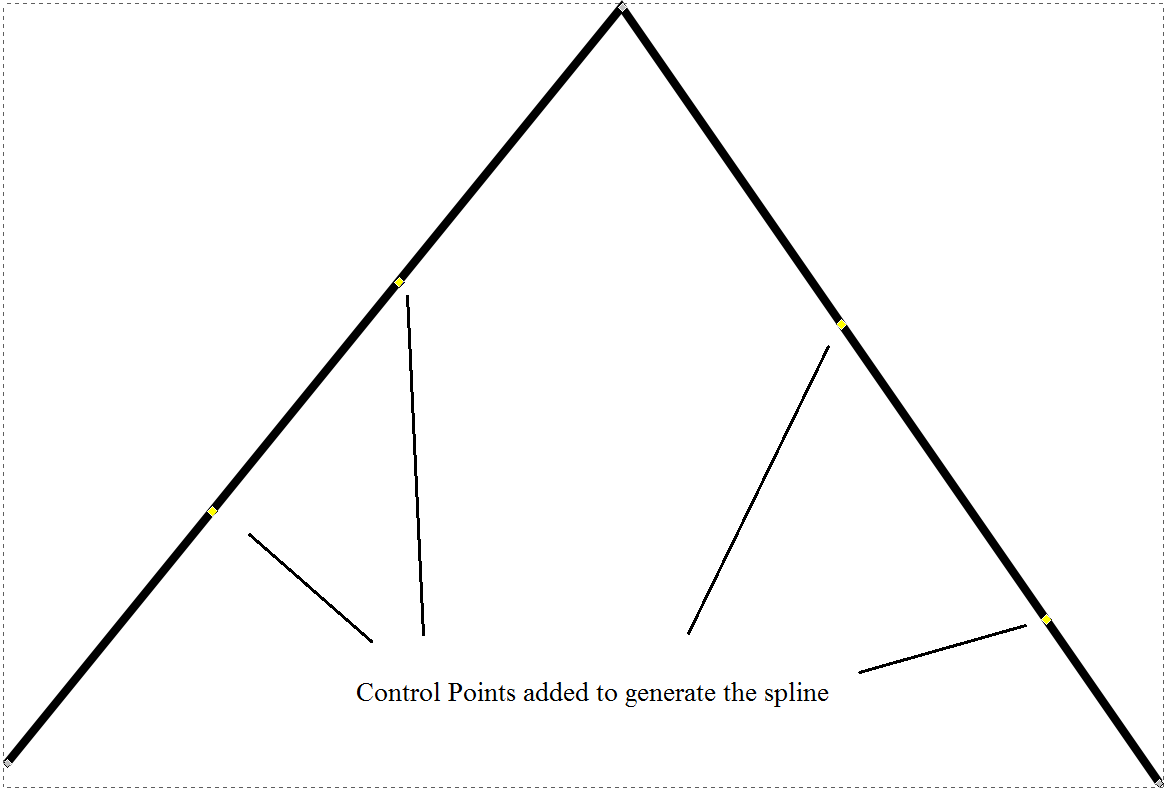
\includegraphics[width=0.48\linewidth]{./images/Smooth1.png}
	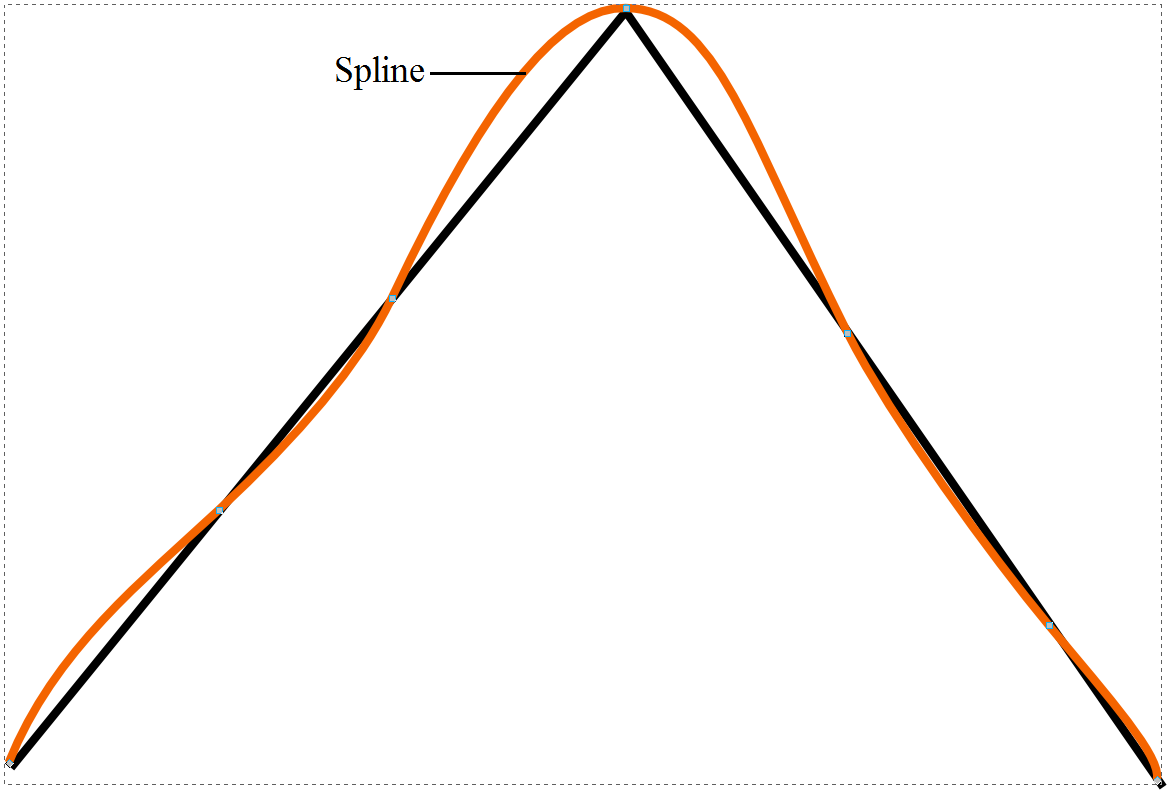
\includegraphics[width=0.48\linewidth]{./images/Smooth2.png}\\
	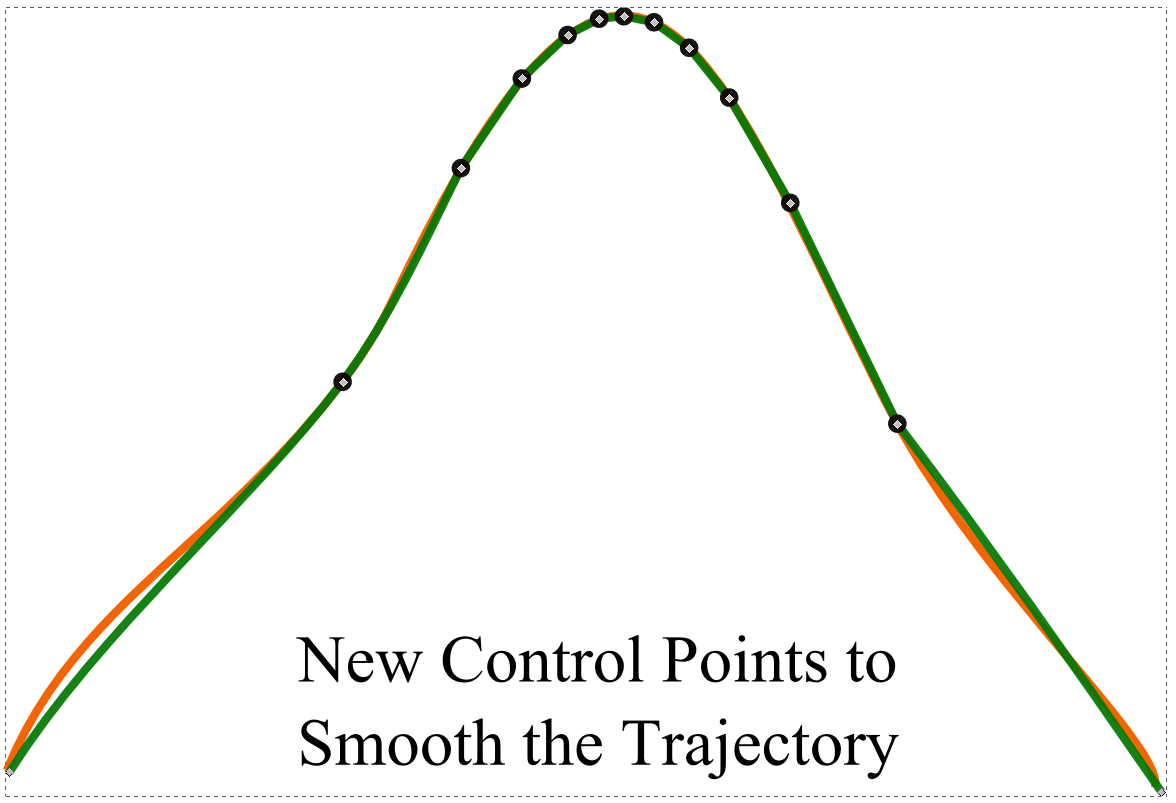
\includegraphics[width=0.48\linewidth]{./images/Smooth3.png}
	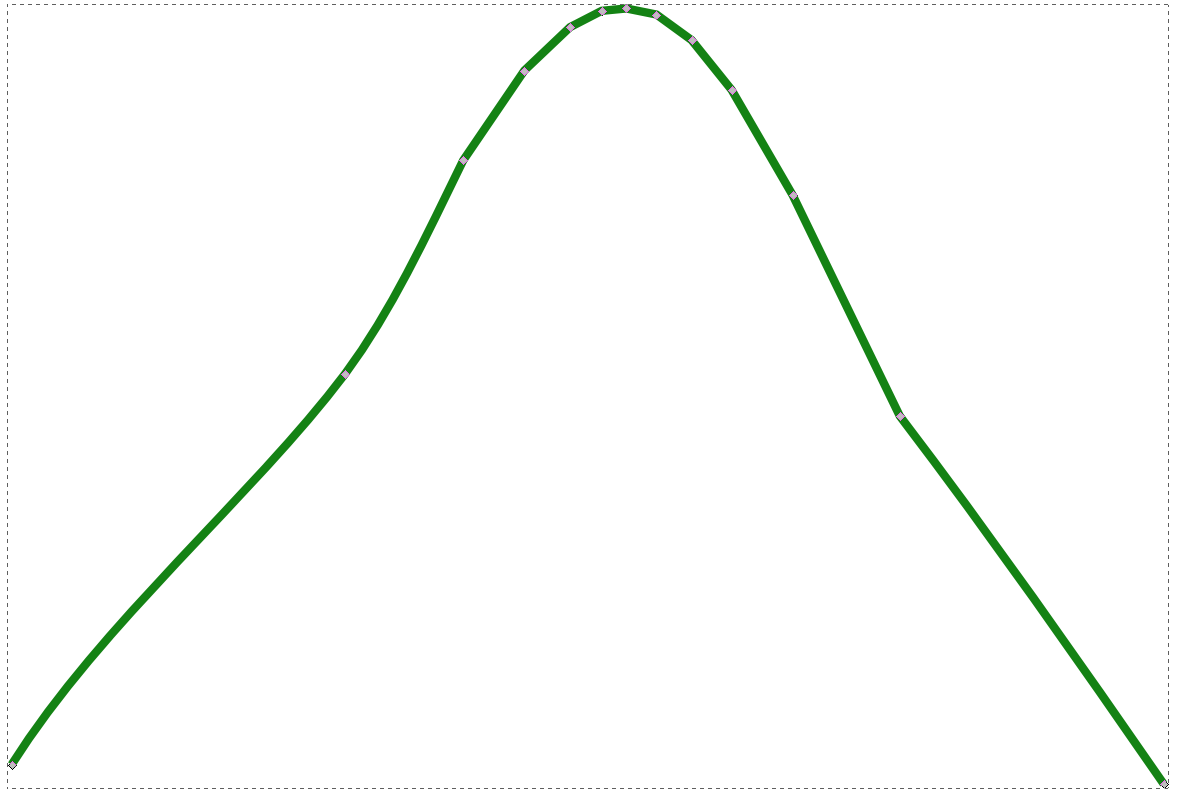
\includegraphics[width=0.48\linewidth]{./images/Smooth4.png}
	\caption{
		\textbf{\textbf{Smoothing Proccess}}
	}
	\label{fig:smoothing}
	\end{center}
\end{figure}
%%-------------------------------------------------------------------
%% Removing collisions figure
%%-------------------------------------------------------------------



There may be cases, even with a healthy number of tacks, that the splines still vary too much from the original trajectory. We define a threshold based on the same threshold of collision to know how far a way a point can be moved. For these cases where the new control point surpasses the threshold, we simply donӴ add it to the set of new control points.  There may be extreme cases (for example, due to too a bad sampling of the tacks at the beginning), where the spline has extreme curves that are very different from our initial trajectory. In those extreme cases most of the new control points would not be added and the new smooth trajectory would end up being very similar to the original one.

Having splines for trajectories is better than having simple straight lines, but we know humans donӴ  follow either of them when walking,  so other methods can be tried to improve this initial approach.


